\documentclass[a4paper, 12pt]{article}

% Для многоязычности
\usepackage{polyglossia}
\setdefaultlanguage[indentfirst=true,spelling=modern]{russian}
\setotherlanguage{english}
% Юникодные математические символы
\usepackage{unicode-math}

\usepackage{amsmath}

\usepackage{fontspec}
% Подключаем шрифт. Шрифт есть в дистрибутиве TeXLive
\setmainfont[Ligatures={Common,TeX},Scale=0.94]{IBM Plex Serif}
\setromanfont[Ligatures={Common,TeX},Scale=0.94]{IBM Plex Serif}
\setsansfont[Ligatures={Common,TeX},Scale=MatchLowercase,Scale=0.94]{IBM Plex Sans}
\setmonofont[Scale=MatchLowercase,Scale=0.94,FakeStretch=0.9]{IBM Plex Mono}

% Математический шрифт
\setmathfont{STIX Two Math}

\usepackage{setspace}
\onehalfspacing

\usepackage[backend=biber,sorting=none]{biblatex}
\addbibresource{bib/cite.bib}

% Пакет для подключения картинок
\usepackage{graphicx}
% Пакет для ссылок (hyper references)
\usepackage{hyperref}

\usepackage{listings}
\usepackage{xcolor}
\lstdefinestyle{mystyle}{
    backgroundcolor=\color{black!5},
    commentstyle=\color{green!40!black},
    keywordstyle=\color{magenta},
    stringstyle=\color{purple},
    basicstyle=\footnotesize\ttfamily,
    numbers=left,
    breaklines=true,
    numberstyle=\tiny\color{black!60},
    frame=tb,
    framerule=0pt,
}
\lstset{style=mystyle}

\usepackage{float}



\renewcommand{\figurename}{Рис.}
\renewcommand{\tablename}{Таблица}
\renewcommand{\lstlistingname}{Листинг}
\renewcommand{\contentsname}{Содержание}
\renewcommand{\listfigurename}{Список иллюстраций}
\renewcommand{\listtablename}{Список таблиц}
\renewcommand{\lstlistlistingname}{Список листингов}

\usepackage{geometry}
\geometry{left=2.5cm, right=1.5cm, top=2cm, bottom=2cm}

\author{Николаев Дмитрий Иванович, НПМмд-02-24}
\title{Лабораторная работа №3: Набор математических формул в \LaTeX \\ Computer Skills for Scientific Writing}
\date{\today}

% Для компиляции выполнить pdflatex main.tex

\begin{document}
  \maketitle
  \tableofcontents
  \pagebreak

  \listoffigures
  %\listoftables
  \lstlistoflistings
  \pagebreak

\section{Цель работы}
Целью данной работы является освоение базовых и расширенных средств \LaTeX для набора математических формул. В ходе работы необходимо научиться использовать различные математические режимы, верстать одиночные и многострочные уравнения, применять выравнивание, создавать матрицы и использовать специализированные стили шрифтов для математических символов.

\section{Теоретическое введение}
Набор математических формул является одной из сильнейших сторон системы вёрстки \LaTeX. В отличие от текстовых процессоров с визуальным редактированием, \LaTeX позволяет логически описывать структуру формул, а система сама заботится об их корректном и эстетичном отображении. Основные инструменты для работы с математикой описаны в пособии~\cite{lab}.

Работа с математикой в \LaTeX строится на двух основных режимах:
\begin{enumerate}
    \item \textbf{Внутристрочный (inline mode)}: для коротких формул, являющихся частью текста. Активируется символами \texttt{\$...\$}.
    \item \textbf{Выключной (display mode)}: для крупных формул, которые выносятся на отдельную строку и центрируются. Активируется конструкцией \texttt{\backslash[...\backslash]} или \texttt{\$\$...\$\$} или специализированными окружениями, такими как \texttt{equation} для нумерованных формул.
\end{enumerate}
Для работы со сложными структурами, такими как системы уравнений или матрицы, используется пакет \texttt{amsmath}, который значительно расширяет стандартные возможности \LaTeX.

\section{Выполнение лабораторной работы}

\subsection{Часть 1: Основы математических режимов}
На первом этапе была создана базовая структура документа \texttt{lab3.tex} и добавлены примеры формул во внутристрочном и выключном режимах.

\paragraph{Вставка формул.}
Были добавлены внутристрочные формулы, выключная формула (интеграл) и его нумерованный аналог. Код для этой части представлен в \lstlistingname~\ref{lst:part1}.

\begin{lstlisting}[
    float=htbp,
    language=tex,
    caption={Код для базовых математических режимов},
    label=lst:part1
]
A sentence with inline mathematics: \(y = mx + c\).

A second sentence with inline mathematics:
$5^{2}=3^{2}+4^{2}$.

A second paragraph containing display math.
\[
y = mx + c
\]
See how the paragraph continues after the display.

Superscripts $a^{b}$ and subscripts $a_{b}$.

Some mathematics: $y = 2 \sin^2 \theta^{2}$.

A paragraph about a larger equation
\[
\int_{-\infty}^{+\infty} e^{-x^2} \, dx
\]

A paragraph about a larger equation (with new operator definition)
\[
\int_{-\infty}^{+\infty} e^{-x^2} \diff x
\]

A paragraph about a larger equation
\begin{equation}
\int_{-\infty}^{+\infty} e^{-x^2} \diff x
\end{equation}
\end{lstlisting}

\paragraph{Компиляция.}
Документ был скомпилирован командой \texttt{pdflatex lab3.tex}. Результат показан на \figurename~\ref{fig:001}: внутристрочные формулы корректно вписаны в текст, выключная формула отцентрирована без номера, а формула в окружении \texttt{equation} получила автоматический номер.

\begin{figure}[H]
    \centering
    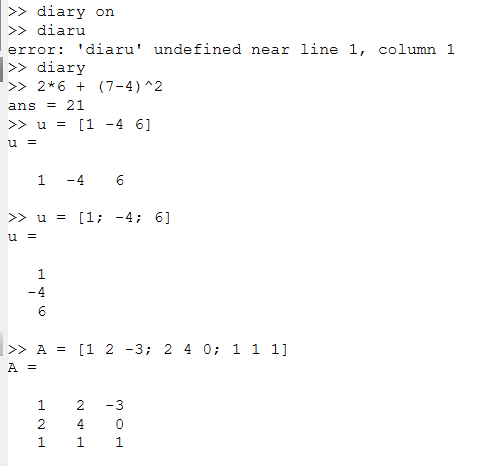
\includegraphics[width=0.8\textwidth]{image/1.png}
    \caption{Результат компиляции первой части работы}
    \label{fig:001}
\end{figure}

\subsection{Часть 2: Расширенные возможности с пакетом amsmath}
В преамбулу документа был добавлен пакет \texttt{amsmath}. С его помощью были свёрстаны система рекуррентных соотношений и несколько матриц.

\paragraph{Использование align* и матриц.}
Окружение \texttt{align*} позволило выровнять уравнения по знаку равенства с помощью символа \texttt{\&}. Окружения \texttt{matrix}, \texttt{pmatrix} и \texttt{bmatrix} были использованы для создания матриц без скобок, в круглых и квадратных скобках соответственно. Итоговый код показан в \lstlistingname~\ref{lst:part2}.

\begin{lstlisting}[
    float=htbp,
    language=tex,
    caption={Код с использованием окружений из amsmath},
    label=lst:part2
]
Solve the following recurrence for $ n,k\geq 0 $:
\begin{align*}
Q_{n,0} &= 1 \quad Q_{0,k} = [k=0]; \\
Q_{n,k} &= Q_{n-1,k}+Q_{n-1,k-1}+\binom{n}{k},
\quad\text{for $n$, $k>0$.}
\end{align*}

AMS matrices.
\[
\begin{matrix}
a & b & c \\
d & e & f
\end{matrix}
\quad
\begin{pmatrix}
a & b & c \\
d & e & f
\end{pmatrix}
\quad
\begin{bmatrix}
a & b & c \\
d & e & f
\end{bmatrix}
\]
\end{lstlisting}
Результат компиляции этой части приведён на \figurename~\ref{fig:002}.

\begin{figure}[H]
    \centering
    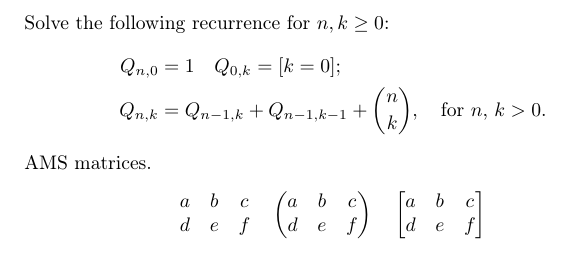
\includegraphics[width=0.8\textwidth]{image/2.png}
    \caption{Система уравнений и матрицы, свёрстанные с помощью amsmath}
    \label{fig:002}
\end{figure}

\subsection{Часть 3: Стили шрифтов в формулах}
Были рассмотрены команды для изменения стиля шрифта внутри математического режима, такие как \texttt{\textbackslash mathbf} для полужирного, \texttt{\textbackslash mathit} для курсива и \texttt{\textbackslash mathrm} для прямого начертания (\lstlistingname~\ref{lst:part3} и \figurename~\ref{fig:003}).

\begin{lstlisting}[
    float=htbp, 
    language=tex,
    caption={Примеры использования стилей математических шрифтов}, 
    label=lst:part3
]
The matrix $\mathbf{M}$ (for comparison $M$).

$\text{bad use } size \neq \mathit{size} \neq \mathrm{size} $

\textit{$\text{bad use } size \neq \mathit{size} \neq \mathrm{size} $}
\end{lstlisting}

\begin{figure}[H]
    \centering
    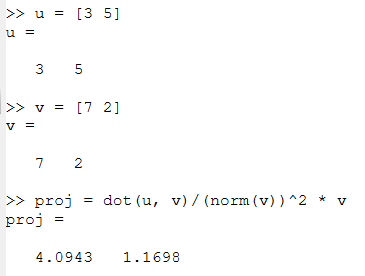
\includegraphics[width=0.8\textwidth]{image/3.png}
    \caption{Разница в отображении различных шрифтов}
    \label{fig:003}
\end{figure}

\subsection{Часть 4: Многострочные формулы}
Для вёрстки сложных многострочных конструкций были применены окружения \texttt{gather} (для группировки формул без выравнивания), \texttt{multline*} (для разбиения одной длинной формулы) и \texttt{align*} (для создания нескольких колонок с выровненными уравнениями). Код приведёт в \lstlistingname~\ref{lst:part4}, а результат представлен на \figurename~\ref{fig:004}

\begin{lstlisting}[
    float=htbp, 
    language=tex,
    caption={Окружения для работы с многострочными формулами}, 
    label=lst:part4
]
Gather
\begin{gather}
P(x)=ax^{5}+bx^{4}+cx^{3}+dx^{2}+ex +f\\
x^2+x=10
\end{gather}
Multline
\begin{multline*}
(a+b+c+d)x^{5}+(b+c+d+e)x^{4} + \\
+(c+d+e+f)x^{3}+(d+e+f+a)x^{2}+(e+f+a+b)x + \\
+ (f+a+b+c)
\end{multline*}

Aligned equations
\begin{align*}
a &= b+1 & c &= d+2 & e &= f+3 \\
r &= s^{2} & t &=u^{3} & v &= w^{4}
\end{align*}

\begin{itemize}
\item
$\begin{aligned}[t]
a&=b\\
c&=d
\end{aligned}$
\item
$\begin{aligned}
a&=b\\
c&=d
\end{aligned}$
\end{itemize}
\end{lstlisting}

\begin{figure}[H]
    \centering
    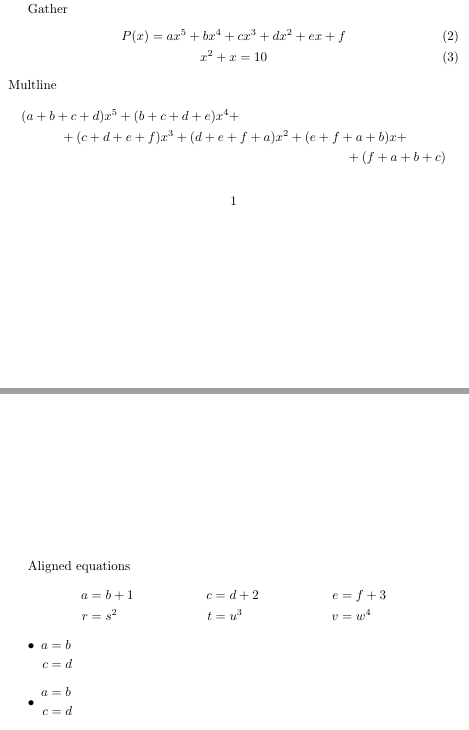
\includegraphics[width=0.8\textwidth]{image/4.png}
    \caption{Различные окружения для многострочных формул}
    \label{fig:004}
\end{figure}

\subsection{Часть 5: Полужирное начертание}
Было проведено сравнение различных способов получения полужирного начертания: команды \texttt{\textbackslash boldmath}, негибкой команды \texttt{\textbackslash mathbf} и наиболее универсальной команды \texttt{\textbackslash bm} из одноимённого пакета (\lstlistingname~\ref{lst:part5} и \figurename~\ref{fig:005}).

\begin{lstlisting}[
    float=htbp, 
    language=tex,
    caption={Сравнение способов получения полужирного начертания}, 
    label=lst:part5
]
Some "bold" math
$(x+y)(x-y)=x^{2}-y^{2}$

{\boldmath $(x+y)(x-y)=x^{2}-y^{2}$ $\qquad \qquad \pi r^2$}

$(x+\mathbf{y})(x-\mathbf{y})=x^{2}-{\mathbf{y}}^{2}$

$\mathbf{\pi} r^2$ - not successful use. % bad use of \mathbf

With bm packet
$$(x+\mathbf{y})(x-\mathbf{y})=x^{2}-{\mathbf{y}}^{2}$$

$$(x+\bm{y})(x-\bm{y}) \bm{=} x^{2}-{\bm{y}}^{2}$$

$$\alpha + \bm{\alpha} < \beta + \bm{\beta}$$
\end{lstlisting}

\subsection{Часть 6: Возможности пакета mathtools}
Пакет \texttt{mathtools} расширяет возможности \texttt{amsmath}. В качестве примера было использовано окружение \texttt{pmatrix*} для создания матрицы в круглых скобках с выравниванием колонок по правому краю (\lstlistingname~\ref{lst:part6} и \figurename~\ref{fig:005}).

\begin{lstlisting}[
    float=htbp, 
    language=tex,
    caption={Выравнивание колонок в матрице с помощью mathtools}, 
    label=lst:part6
]
mathtolls alignment
\[
\begin{pmatrix*}[r]
10000&11\\
1&2\\
-5&-6
\end{pmatrix*}
\]
\end{lstlisting}

\begin{figure}[H]
    \centering
    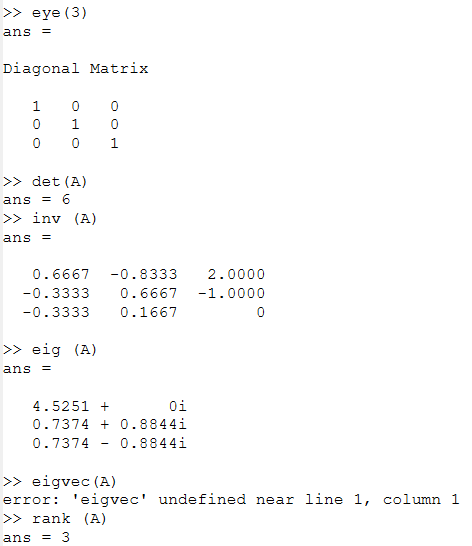
\includegraphics[width=0.8\textwidth]{image/5.png}
    \caption{Сравнение разных полужирных начертаний в формулах и выравнивание в матрице}
    \label{fig:005}
\end{figure}

\subsection{Часть 7: Специализированные символы и ссылки}
Для вставки специальных символов, таких как готический (`\backslash mathfrak`), рукописный (`\backslash mathscr`) и ажурный (`\backslash mathbb`), были подключены соответствующие пакеты. Также была продемонстрирована работа перекрёстных ссылок на нумерованные формулы с помощью команд `\label` и `\eqref`. Код приведёт в \lstlistingname~\ref{lst:part7}, а результат представлен на \figurename~\ref{fig:006}

\begin{lstlisting}[
    float=htbp, 
    language=tex,
    caption={Специальные символы и перекрёстные ссылки}, 
    label=lst:part7
]
One two three
\[
\log \alpha + \log \beta = \log(\alpha\beta)
\]

Unicode Math Alphanumerics
\[A + \symfrak{A}+\symbf{A}+ \symcal{A} + \symscr{A}+\symbb{A}\]


%---------------------------------

See~\eqref{eq_my}
\begin{equation}\label{eq_my}
\gamma + \symbf{\delta_{\symfrak{D}}^{\symcal{\varepsilon}}} = \symbb{DE}_{\symscr{\omega}}
\end{equation}
\end{lstlisting}

\begin{figure}[H]
    \centering
    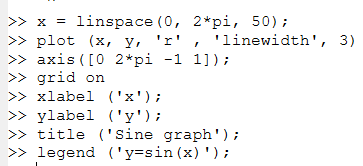
\includegraphics[width=0.8\textwidth]{image/6.png}
    \caption{Проверка различных специальных символов и начертаний из unicode-math}
    \label{fig:006}
\end{figure}

Дополнительно было составлено выражение с комбинацией различных шрифтов, откуда стало ясно (см.~\figurename~\ref{fig:007}), что работает самый последний, внутренний указатель на шрифт.

\begin{figure}[H]
    \centering
    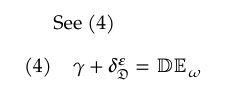
\includegraphics[width=0.8\textwidth]{image/7.png}
    \caption{Проверка вложенности различных шрифтов}
    \label{fig:007}
\end{figure}

\section{Итоговый результат}
В заключительной части было изучено влияние опции класса документа \texttt{fleqn} и \texttt{leqno}. В итоге, был получен финальный документ, в котором все выключные формулы вместо центрирования они стали выравниваться по левому краю с небольшим отступом, и с того же левого края отображаются номера формул. Весь код приведён в \lstlistingname~\ref{lst:final_code}, а результат его компиляции --- на \figurename~\ref{fig:008_1}--~\ref{fig:008_2}.


\begin{lstlisting}[
    %float=htbp, 
    %allowpagebreak,
    language=tex,
    caption={Полный исходный код файла lab3.tex}, 
    label=lst:final_code
]
\documentclass[fleqn,leqno]{article}
\usepackage[T1]{fontenc}
\usepackage{amsmath}
\usepackage{bm}
\usepackage{mathtools}

\usepackage{unicode-math}
\setmainfont{TeX Gyre Pagella}
\setmathfont{TeX Gyre Pagella Math}
%\newcommand{\diff}{\mathop{}\!d} % For italic
\newcommand{\diff}{\mathop{}\!\mathrm{d}} % For upright

\begin{document}

A sentence with inline mathematics: \(y = mx + c\).

A second sentence with inline mathematics:
$5^{2}=3^{2}+4^{2}$.

A second paragraph containing display math.
\[
y = mx + c
\]
See how the paragraph continues after the display.

Superscripts $a^{b}$ and subscripts $a_{b}$.

Some mathematics: $y = 2 \sin^2 \theta^{2}$.

A paragraph about a larger equation
\[
\int_{-\infty}^{+\infty} e^{-x^2} \, dx
\]

A paragraph about a larger equation (with new operator definition)
\[
\int_{-\infty}^{+\infty} e^{-x^2} \diff x
\]

A paragraph about a larger equation
\begin{equation}
\int_{-\infty}^{+\infty} e^{-x^2} \diff x
\end{equation}

%------------------------------

Solve the following recurrence for $ n,k\geq 0 $:
\begin{align*}
Q_{n,0} &= 1 \quad Q_{0,k} = [k=0]; \\
Q_{n,k} &= Q_{n-1,k}+Q_{n-1,k-1}+\binom{n}{k},
\quad\text{for $n$, $k>0$.}
\end{align*}

AMS matrices.
\[
\begin{matrix}
a & b & c \\
d & e & f
\end{matrix}
\quad
\begin{pmatrix}
a & b & c \\
d & e & f
\end{pmatrix}
\quad
\begin{bmatrix}
a & b & c \\
d & e & f
\end{bmatrix}
\]

%---------------------------------

The matrix $\mathbf{M}$ (for comparison $M$).

$\text{bad use } size \neq \mathit{size} \neq \mathrm{size} $

\textit{$\text{bad use } size \neq \mathit{size} \neq
\mathrm{size} $}

%---------------------------------

Gather
\begin{gather}
P(x)=ax^{5}+bx^{4}+cx^{3}+dx^{2}+ex +f\\
x^2+x=10
\end{gather}
Multline
\begin{multline*}
(a+b+c+d)x^{5}+(b+c+d+e)x^{4} + \\
+(c+d+e+f)x^{3}+(d+e+f+a)x^{2}+(e+f+a+b)x + \\
+ (f+a+b+c)
\end{multline*}

Aligned equations
\begin{align*}
a &= b+1 & c &= d+2 & e &= f+3 \\
r &= s^{2} & t &=u^{3} & v &= w^{4}
\end{align*}

\begin{itemize}
\item
$\begin{aligned}[t]
a&=b\\
c&=d
\end{aligned}$
\item
$\begin{aligned}
a&=b\\
c&=d
\end{aligned}$
\end{itemize}

%---------------------------------

Some "bold" math
$(x+y)(x-y)=x^{2}-y^{2}$

{\boldmath $(x+y)(x-y)=x^{2}-y^{2}$ $\qquad \qquad \pi r^2$}

$(x+\mathbf{y})(x-\mathbf{y})=x^{2}-{\mathbf{y}}^{2}$

$\mathbf{\pi} r^2$ - not successful use. % bad use of \mathbf

With bm packet
$$(x+\mathbf{y})(x-\mathbf{y})=x^{2}-{\mathbf{y}}^{2}$$

$$(x+\symbf{y})(x-\symbf{y}) \symbf{=} x^{2}-{\symbf{y}}^{2}$$

$$\alpha + \symbf{\alpha} < \beta + \symbf{\beta}$$

%---------------------------------

mathtolls alignment
\[
\begin{pmatrix*}[r]
10000&11\\
1&2\\
-5&-6
\end{pmatrix*}
\]

%---------------------------------

One two three
\[
\log \alpha + \log \beta = \log(\alpha\beta)
\]

Unicode Math Alphanumerics
\[A + \symfrak{A}+\symbf{A}+ \symcal{A} + \symscr{A}+\symbb{A}\]


%---------------------------------

See~\eqref{eq_my}
\begin{equation}\label{eq_my}
\gamma + \symbf{\delta_{\symfrak{D}}^{\symcal{\varepsilon}}} = \symbb{DE}_{\symscr{\omega}}
\end{equation}

\end{document}
\end{lstlisting}

\begin{figure}[H]
    \centering
    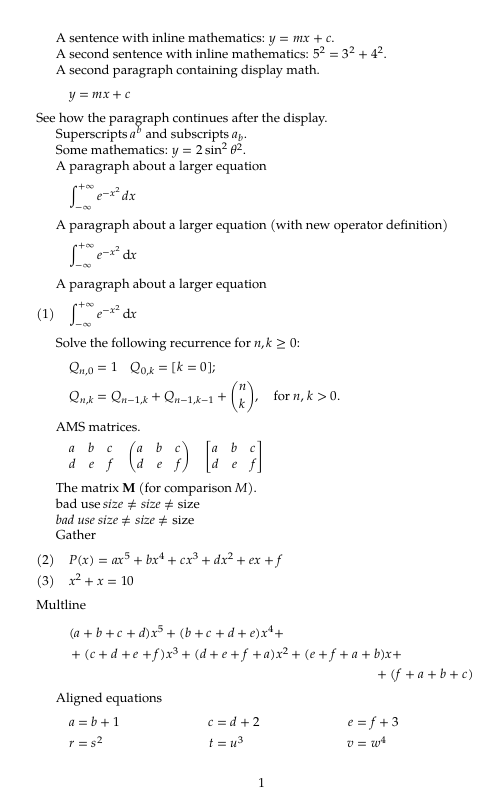
\includegraphics[width=0.8\textwidth]{image/8_1.png}
    \caption{Итоговый результат 1}
    \label{fig:008_1}
\end{figure}

\begin{figure}[H]
    \centering
    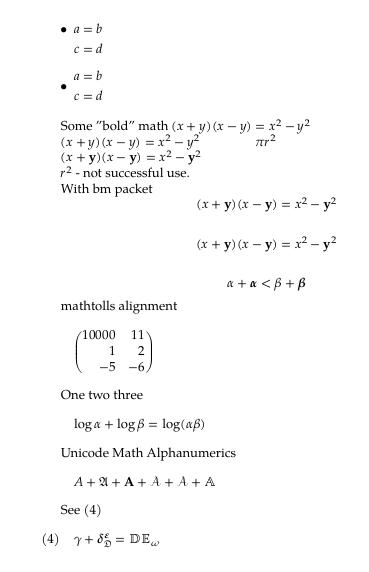
\includegraphics[width=0.8\textwidth]{image/8_2.png}
    \caption{Итоговый результат 2}
    \label{fig:008_2}
\end{figure}

\section{Выводы}
В ходе выполнения данной лабораторной работы я освоил ключевые инструменты LaTeX для набора математических формул. Были изучены как базовые математические режимы, так и расширенные возможности, предоставляемые пакетом \texttt{amsmath}, включая окружения для выравнивания (\texttt{align*}), группировки (\texttt{gather}), разбиения длинных формул (\texttt{multline*}) и создания матриц. Также я научился управлять стилями математических шрифтов и изменять глобальные настройки выравнивания формул в документе.

%\nocite{*}
\printbibliography
  
\end{document}